The goal of the HAEC project is to demonstrate secure forward facing network services using trusted enclaves. We believe\cite{Zaber_Nair_Medamana_Krinos_Cepleanu} that securing attachment points and edge components is a primary concern for modern network architectures. To allow for agile experimentation under different scenarios, we have deployed a laboratory environment based on open networking standards and implementations including OpenFlow, ONOS, ONIE, and ONAP. 3 Intel NUC8i7BEH with 32G DDR each provide trusted enclave implementations for the edge compute experiments. It has been shown\cite{sgx-lkl_2018} that enclave execution incurs ~15\%-25\% overhead, so performance for CPU bound deployments is a consideration. 

\begin{figure}[H]
\centering
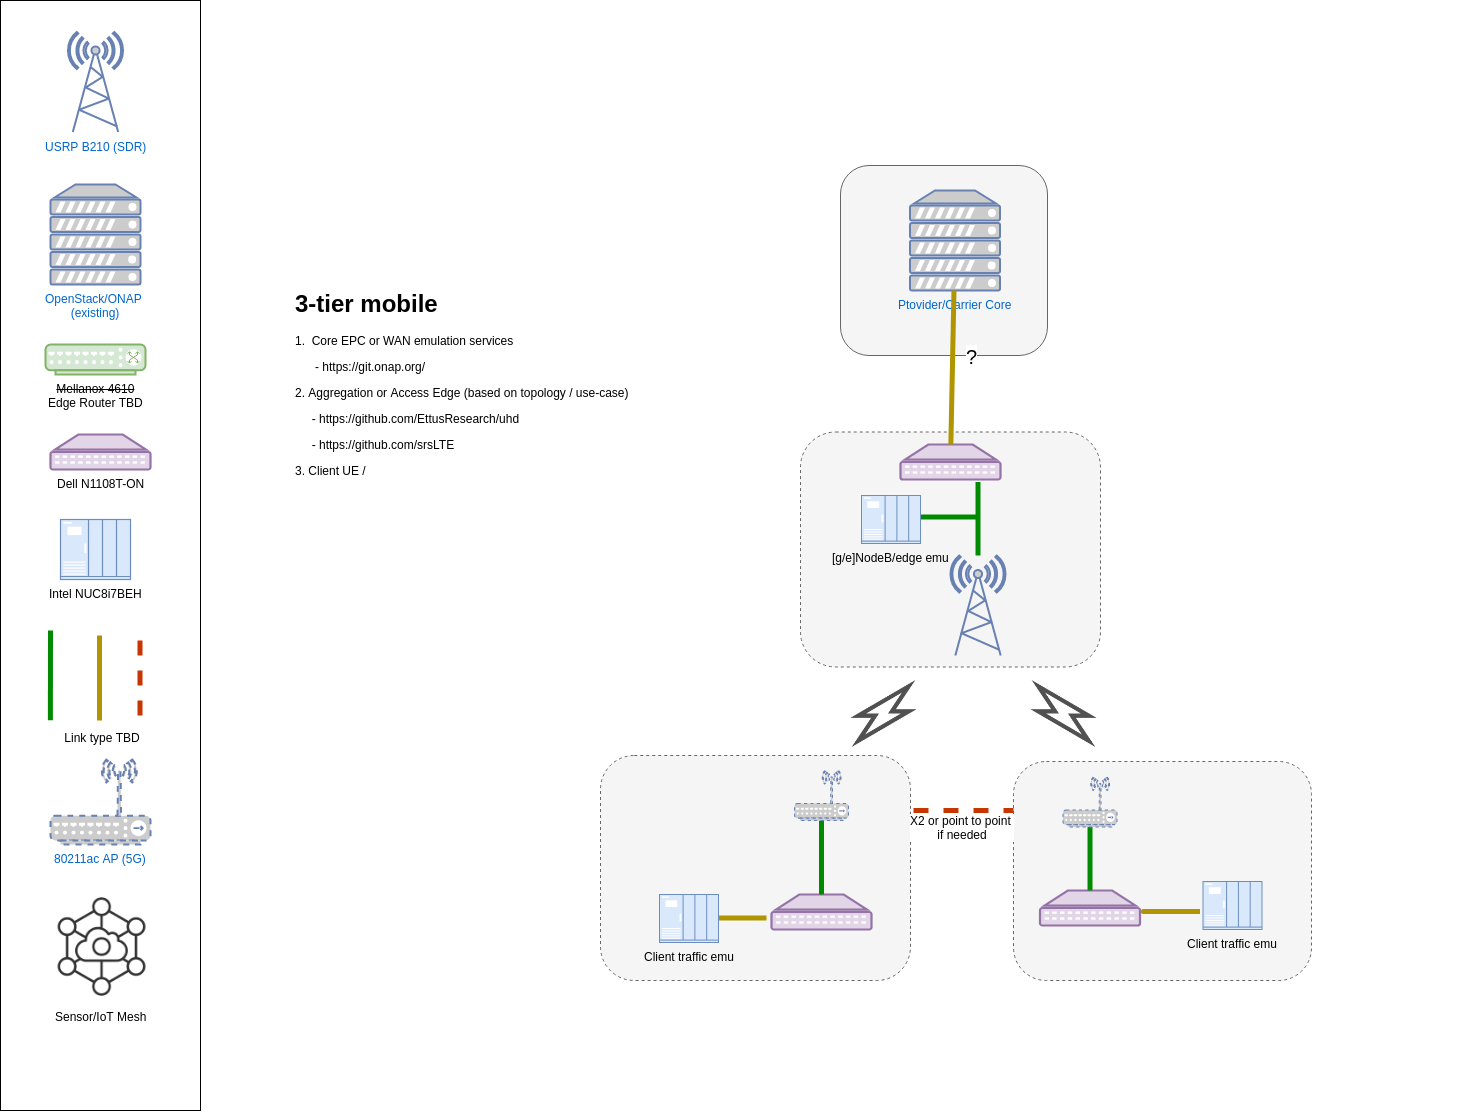
\includegraphics[scale=.3]{img/net_archs/mec_arch_3tier.png}
\caption{MEC 3-tier architecture}
\label{fig:mec_3tier}
\end{figure} 

\begin{figure}[H]
\centering
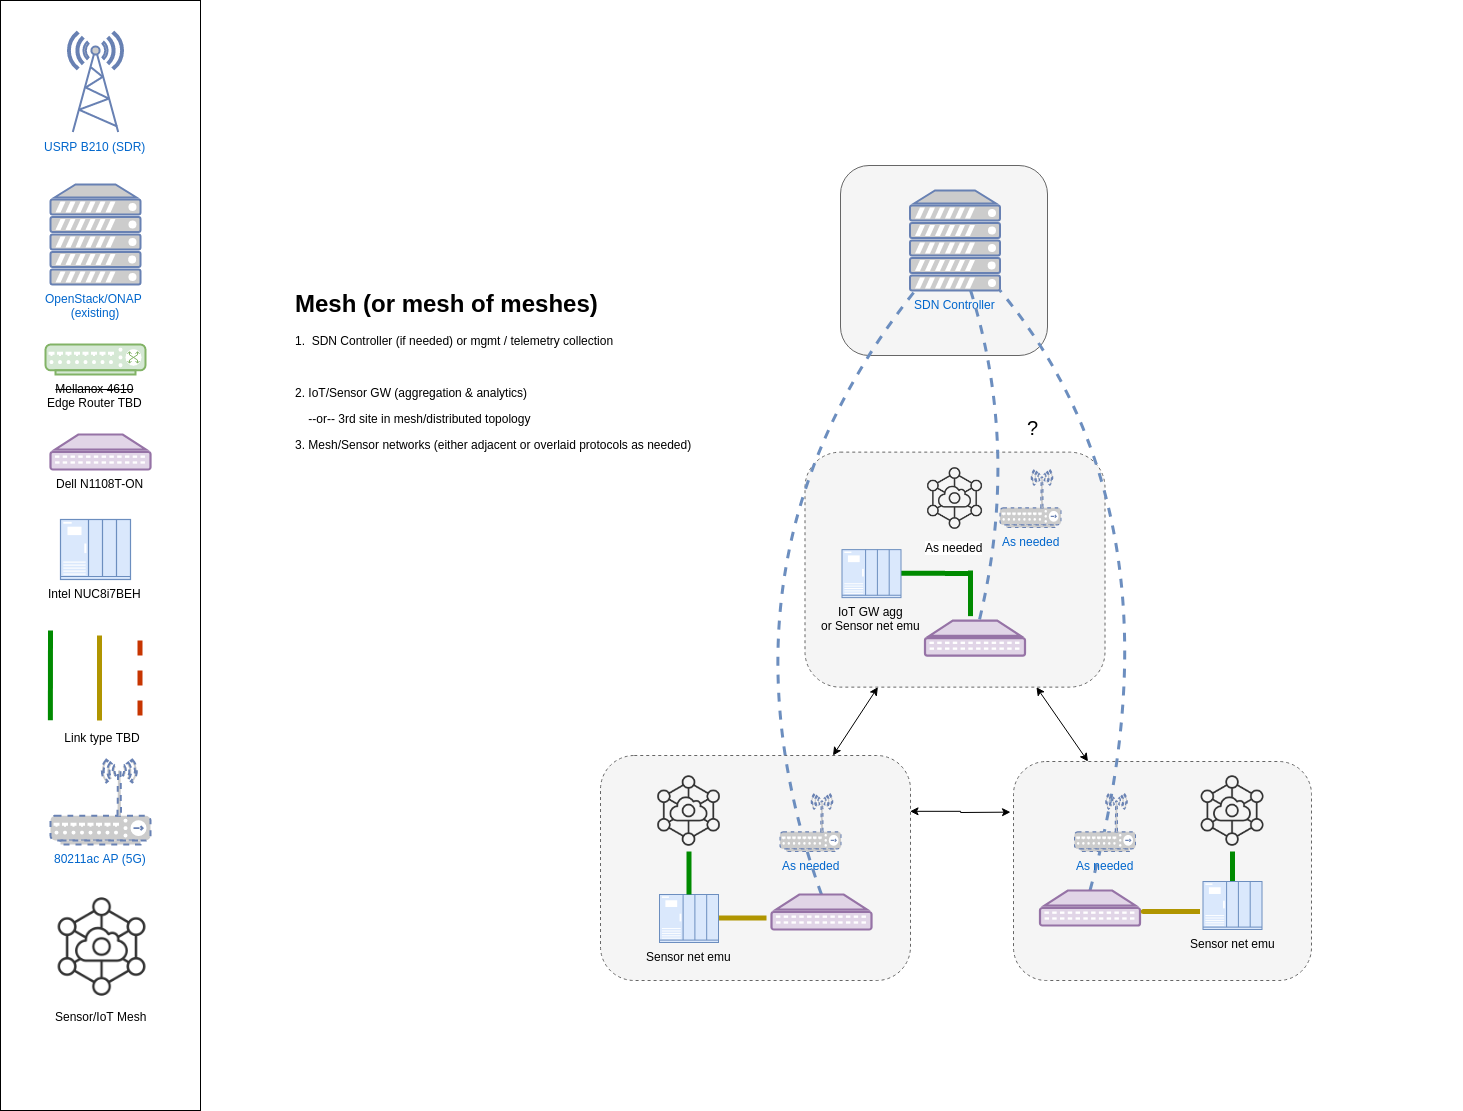
\includegraphics[scale=.3]{img/net_archs/mec_arch_mesh_of_mesh.png}
\caption{MEC mesh architecture}
\label{fig:mec_mesh}
\end{figure}

To demonstrate an application of HAEC, we consider a stream processing use case. The streams being processed could be sensor data, formatted logs, or some other continuously updated data source... but for our tests we simply run benchmarks like YCSB or known text topologies like word count for validation. 